\chapter{The cross-platform compendium creation methodology and COMMAND 
system}\label{ch:command}
\chaptermark{Command}

\ldots

\instructionsintroduction

\section{Introduction}

Microarrays are one of the main technologies for large-scale transcriptional 
gene expression profiling. 
To promot data sharing, scientific journals generally require the 
deposit of these high-throughput experiments in public databases, such as Gene 
Expression Omnibus (GEO) \cite{Barrett2011} or ArrayExpress 
\cite{Parkinson2009}, upon publication. 
These databases are an extremely rich source of information, containing freely 
accessible data for thousands of experiments and a multitude of different 
organisms, and in theory provide an opportunity to analyse gene expression of a 
particular species at a global level. 
They hold the potential to expand the scope of any smaller scale study: 
mining the information contained in such databases offers molecular biologists 
the possibility to view their own dedicated experiments and analysis in light 
of what is already available. 
So far however, this wealth of public information remains largely untapped 
because these databases do not allow for a direct and integrated exploration of 
their data. 
The opportunity of combining all public experiments for a single organism has 
not been explored due to practical issues that can ultimately be attributed to 
the large heterogeneity inherent to microarray data. 
Data sets originate from different experimenters or labs and microarrays do not 
constitute a uniform technology. 
Multiple microarray platforms exist and are manufactured in different ways. 
Even for similar platforms, protocols for sample preparation, labelling, 
hybridization and scanning can vary greatly. 
Although community standards specifying the mandatory minimal experimental 
information accompanying each dataset (e.g., MIAME \cite{Brazma2001}) have been 
long established, the lack of the requirements \cite{Brazma2009} imposed 
regarding the format of the platform descriptions and the expression 
measurements, as well as the degree of preprocessing done on these values 
further complicates the matter of experiment integration from a practical point 
of view. 


Despite such difficulties, several initiatives exist to actively build 
expression compendia from public resources. 
Most existing compendia can roughly be divided in two groups \cite{Fierro2008}: 
those that directly integrate single-platform experiments, and those that 
indirectly integrate cross-platform experiments. 
Combining data from a single platform makes the in-between experiment 
normalization and probe mapping relatively straightforward, so that 
the quantitative measures of gene expression can be analysed directly across 
experiments. 
Most single-platform compendia databases, such as for instance 
M$^{\textrm{3D}}$ \cite{Faith2008}, or the commercial Genevestigator 
\cite{Hruz2008}, focus on Affymetrix, one of the more robust and reproducible 
platforms \cite{Bammler2005, Irizarry2005}. 
Combining data from different platforms, even to the extent of combining data 
from single- and dual-channel microarrays, is generally done by indirect 
meta-analysis as opposed to directly integrating the actual expression values: 
one first applies the desired analysis procedure (e.g., identifying 
differentially expressed genes, clustering gene expression profiles, etc.) on 
each single data set within the compendium separately, and subsequently 
combines the derived results. 
These compendia are often topic-specific, collecting all publicly available 
experimental information related to a subject matter of interest. 
ITTACA \cite{Elfilali2006} and ONCOMINE \cite{Rhodes2007}, for instance, focus 
on cancer in human; Gene Aging Nexus \cite{Pan2007} on aging in several 
species. 
There are exceptions though, such as the large ATLAS \cite{Kapushesky2010} 
initiative from ArrayExpress.


The compendia created by directly integrating data across experiments have the 
advantage of retaining actual expression values, which broadens the scope of 
potential analysis procedures compared to indirect meta-analysis.
Most of such compendia center on eukaryotic organisms, for which considerable 
amounts of data are available. 
Relying on only one platform can still lead to sizeable compendia with a broad 
scope in condition content, such as the human compendium constructed based on 
the Affymetrix U133A platform with over 5000 samples \cite{Lukk2010}. 
However, for most species (e.g., \textit{Zea mays}), no single platform has 
such a dominant role. 
%
The worst is prokaryotes. 
Even for model organisms such as {\it E. coli}, much less data is available on 
individual platform and a significant portion of the data is missed out when 
considering only one platform. 

To have the advantage of the direct integration, while not being limited to a 
single platform, we have devised methodology that directly combines 
expression data across platforms and experiments. 
The methodology has enabled us to create comprehensive compendia incorporating 
most high quality public data covering a broad range of experimental 
conditions as well as extensive types of biological samples. 
To facilitate the creation of new compendium and the curation of the existing 
ones, a software system COMMAND (Cross-platform cOMpendium MANagement Desktop) 
is also developed, utilizing web browser as the front-end and our methodology 
at the back-end. 







\section{Methods}


\todo{COMMAND: reminder to be commented}
\textbf{REMINDER: Hurdles to create cross-platform exp compendium}

There are \textbf{three main hurdles} preventing direct data integration across
platforms and experiments.
%
\begin{itemize}
%
\item[exp-data] The lack of a consistent format to report expression data
  prevents an automatic and computerized data retrieve.
%
  The heterogeneity of microarray platforms hampers direct integration in two
  aspect.  The possible probe sequence differences of a gene across different
  platforms questions the compatibilities of the obtained measurements.
%
\item[metadata] The metadata describing biological sample and experimental
  conditions is provided as free text which is often incomplete and lack of
  consistency.  Standards like MIAMI \cite{Brazma2001, Brazma2009}, although
  promote human interpretation of experimental conditions, do not facilitate
  computational analysis.
%
\item[normalization] The different preprocessing algorithms employed by
  different experiments further complicates the data compatibility.
%
  The log ratio calculation, capable of removing certain technical variations
  from the normalized data, inherently improves the data consistency across
  platforms and experiments \cite{Shi2006, Shi2008}
%
\end{itemize}



\subsection{Cross-platform expression compendion}

Our expression compendium is essentially an organism-specific matrix of
expression values derived from publicly available microarray experiments which
are homogenized to make them comparable.
%
The rows of a compendium correspond to the known genes of the organism in
question constructed based on the corresponding RefSeq file at NCBI
\cite{Pruitt2007}.
%
Uniquely, each column of it is a `\textit{condition contrast}', which does not
represent single biological sample, but in fact always represents the
differences between a pair of samples, one as test and the other reference.
%
Consequently, the expression values themselves are calculated as expression
log-ratios.
%
Converting absolute measurements of expression into expression changes is the
principal means for rendering expression values comparable across platforms and
experiments.
%
Relative expression calculated intra-experiment/platform (i.e. between two
conditions measured in the same microarray experiment using one platform)
negates much of the platform and experiment specific variations that makes it
impossible to reliably compare the absolute quantities reported in different
experiments \cite{Shi2006}.


\subsubsection{The database structure for expression compendium}

\todo{COMMAND: to be finished with a abstract schema in figure,
  Ref. MIAME2001, MIAMEPlant2006}


To facilitate the further explanation, we give several definitions at here. 
%
A gene expression experiment is an experiment where gene expression of a set of 
biological samples are measured. 


experiment
platform
array
hybridization
raw data

sample
contrast
annotation
norm data

gene
gene annotation

\textbf{Hybridization} refer to a biological sample that is hybridized onto a
microarray platform.
%
Note that for single channel platforms, such as Affymetrix, there is only one
hybridization per chip, wherease for dual channel platforms, there are two
hybridizations per chip labelled with different dyes.
%
Although rarely, there could be upto three hybridizations per chip. 




\subsection{The compendion creation methodology}
\label{sec:colombos-comp-method}

\begin{figure}
  \centering
  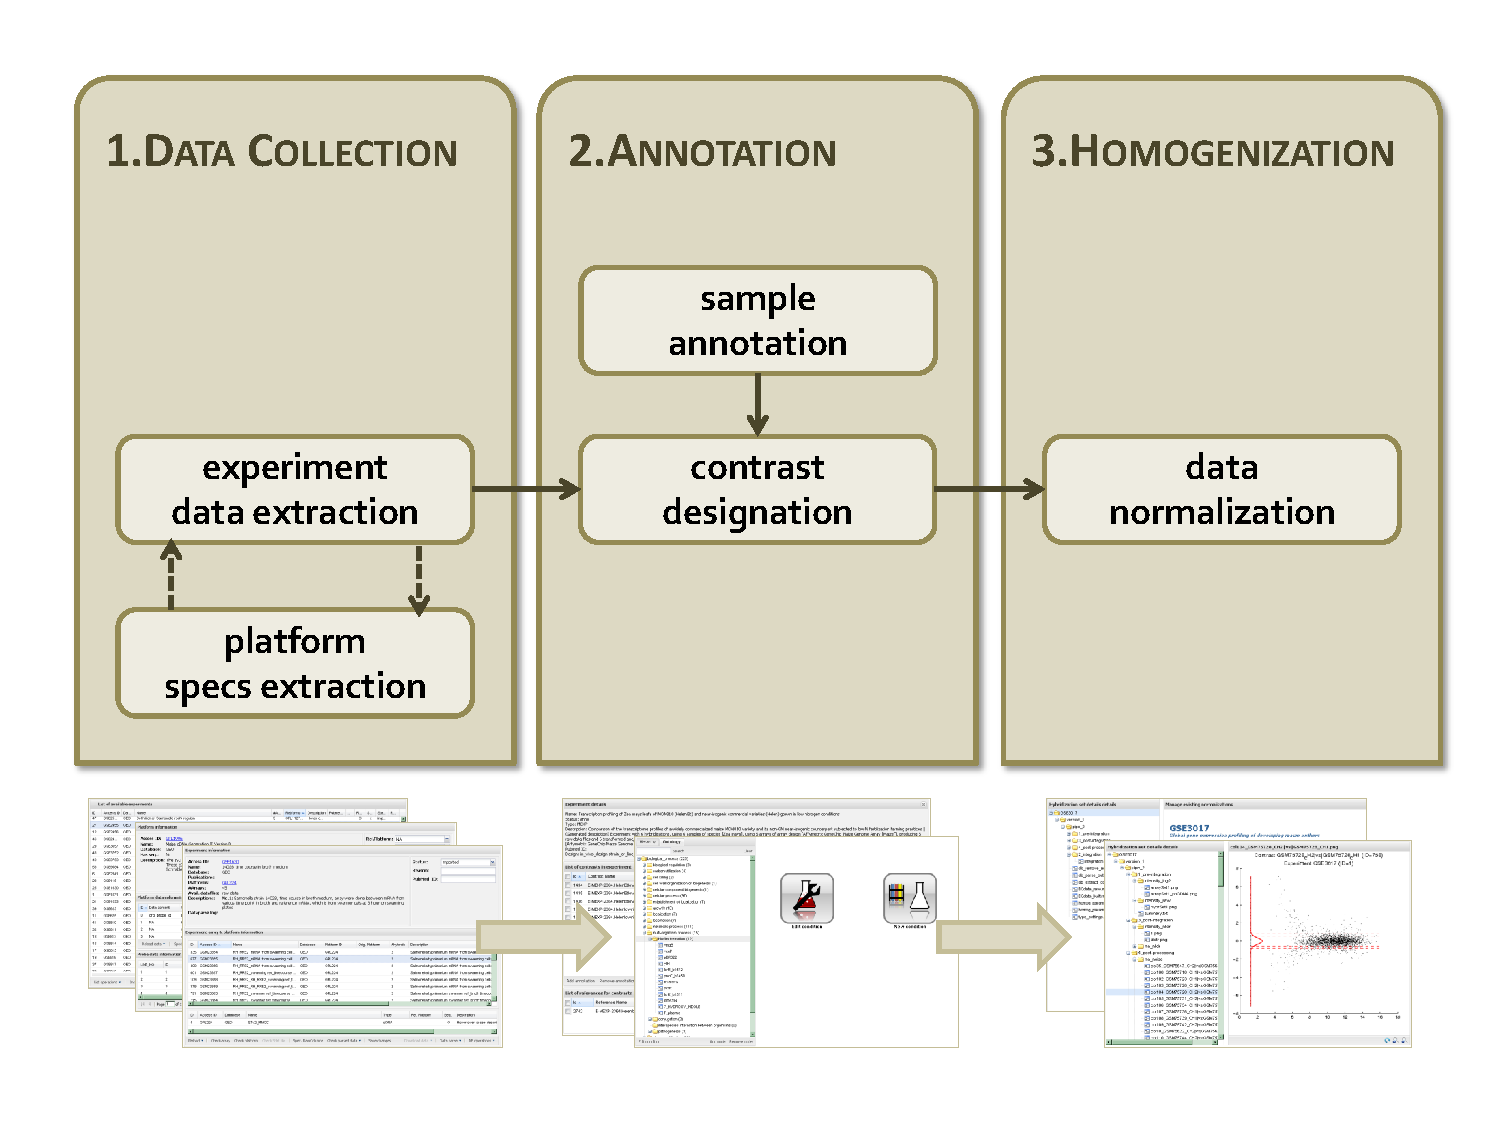
\includegraphics[width=1\textwidth]{COMMAND_Workflow.pdf}
  \caption[Cross-platform expression compendium creation methodology]{
    \textbf{Cross-platform expression compendium creation methodology}.
    From left to right, three box represent three main steps of the 
    cross-platform expression compendium creation methodology. The 
    corresponding functionalities are specified in the rectangles inside of 
    each box. Below the box shown the snapshots of the corresponding COMMAND 
    interfaces.}
  \label{fig:command-workflow}
\end{figure}


The cross-platform compendium creation methodology is composed of three major 
steps (Figure \ref{fig:command-workflow}), namely, data collection, experiment 
annotation, and data homogenization. 
%
%
First, in data collection step, the expression data and the accompany 
(experiment and platform) information are retrieved from the online 
repositories, overcoming the issue of the prevalent data representation 
discrepancies. 
%
Next in annotation step, the contrasts are constructed by assigning a pair of 
samples, one as reference and the other as test. And the experimental 
condition differences between the corresponding samples are 
curated manually and specified for each contrast using a set of in-house 
controlled vocabularies. 
%
At last, the raw expression data are normalized and converted into log 
ratios based on the sample contrast association in data homogenization step, 
creating a cross-platform expression compendium. 
%
%
In the following sections, we will explain the individual step in detail.









\subsubsection{Data collection}

%% Summary
The first step is the retrieval of microarray experiment data and the
associated platforms infromation from online repositories, such as, Gene
Expression Omnibus (GEO), and ArrayExpress.
%
The widespread data discrepancy coupled with the colossal amount of the
publically data available in those repositories makes the systematical
expression data retrieval a daunting task.
%
To make this task viable, we develop a semi-automatic workflow that is
specifically designed to tackle data discrepancies and automates data
process procedures to handle the huge volume of the data.
\todo{COMMAND: need to be adapted.}



\paragraph{Data retrieval goal}
%
There are three types of information to be extracted, the experiment
information, the platform specification, and the (probe) expression
values.
%
\todo{COMMAND: need to be explained in the introduction} The experiment
information describing the sample attributes and experimental factors is
essential for understanding observed gene expression variations.
%
% automated data processing in homogenization, standard format required, 
% discrepencies need to be removed (main task of data retrieval) 
%
As the expression value is measured by individual probe of a microarray,
the measurements are reported for each probe, instead of individual gene.
%
To convert these raw probe measurements into gene expression values, it
is crucial to obtain platform specification containing probe annotation
describing the probe-to-gene correspondence.
%
Additionally, the platform specification also provides clues about the
number of samples hybridized on a microarray providing hints about the
expected amount of data to be retrieved.


Often the expression values directly reported in online reposirtories are
the normalized values.
%
In order to reduce the artificial inconsistency introduced by using
different data normalization algorithms, the raw probe intensity
expression values without background correction are retrieved when
possible.
%
The retrieved data is then normalized in later step utilizing an in-house
pipeline to improve the consistency.




\paragraph{Data discrepancies and the extraction strategy}

\begin{itemize}
\item free text for experimental information
\item lack of standard format to report platform probe specification,
  sequence information is not always provided
\item raw data is not always required, if provided, lack of standard
  format to report raw data
\item lack of number of channels specification for each microarray or
  platform, or alternatively platform type specification
\end{itemize}


Although community guidelines such as MIAME \cite{Brazma2001} exist, they
mainly focus on the content rather than the formality of the reported
information.
%
The lack of a standard data reporting format creates widespread represetation
discrepancies among the data deposite in the online repositories.
%
%% There are three categories of discrepancies exist among the expression data
%% available in online repositories, the discrepancies in specifying platform
%% probe annotations, the discrepancies in reporting expression values, and the
%% discrepancy in connecting expression values with the corresponding probe
%% annotations.
%
This lack of formality and consistency presents itself in several aspects.
%
Below, we will discuss each of those issues and how it is handled in data
collection step.


\subparagraph{First}, the experiment metadata, such as, the sample attributes and
experimental factors, are described using the free text instead of
controlled vocabulary.
%
The free text lacks consistency as often there are multiple possibilities
to describe one concept.
%
This renders a computerized data extraction impossible. Instead, a time
consuming manual curation (in the annotation step) is required to analyze
and standardize these information into a computable format to facilitate
data exploration.
%
Hence, these set of information is extracted in its original form at this
step.


%% - experiment metadata, experimental condition
%% - sample attributes and experimental factors (i.e. conditions under
%%   study) \textbf{ATLAS2013}

%% \textbf{M3D} The fourth obstacle is the incompleteness and
%% inconsistency in the curation of metadata describing the details of
%% each experimental condition. Each expression profile run for a given
%% species can have a different genetic background, media, growth
%% conditions and any number of chemicals, which might have an effect on
%% the cell’s expression. Such data is fundamental to the meaningful
%% interpretation of expression data. Even when provided, this metadata is
%% found as unstructured prose in the database deposit or in the methods
%% sections of each publication. Ideally, this metadata would be collected
%% in a computable format with uniform units across all
%% laboratories. Although standards like MIAME (10) promote the human
%% interpretation of experimental conditions, the standard is unevenly
%% applied and it does not facilitate computational analysis



\subparagraph{Second}, the lack for uniform format to report probe annotation for a
platform.
%
The probe annotation is always presented as a table, nevertheless each
platform has its own format that varies in the amount of content (number
of columns), the column naming convention, and the content of individual
column.
%
Idealy, the probe sequences should be provided so that a homology search
against the lastest gene sequences using BLAST \cite{BLAST} can identify
the up-to-date target gene for each probe.
%
However, though required by MIAME\cite{MIAME} standard, this
information is missing for the majority of the platforms.
%
Alternatively, the target gene can be identified by other information,
namely, locus tags, alternative gene tags, or common gene names.
%
But the lack of a consistent format makes it hard to identify the
corresponding column providing those information.
%
Even worse, sometimes the relevant information is embedded in a column in
which multiple contents are specified in a complicated structure. 
%
For example, locus tag, gene name, or even other gene tags are used
alternatively in one data column titled 'ORF'.
%
Hence it is very difficult to extract them.
%
Furthermore, the content inconsistency exists that different types of
information are found in one data column.

Due to these data issues, a fully automated platform data extraction is
not feasible.
%
Hence a user-guided semi-automatic three-step procedure is used to process
platform data collecting a standard set of information for every platform.
%
In the first step, the platform information is separated from other
information.
%
An in-house dictionary storing common column names, the corresponding most
probable content type, and the most common extraction method is utilized
to automatically mark out the candidate data columns.
%
Next, a manual inspection is required. 
%
The content and the data extraction functions of the automatically marked
columns are checked, and the adjustment is made when necessary to
guarantee the contents are properly extracted.
%
The other columns are checked only when necessary information could not be
obtained from the marked columns.
%
In the last step, the data are then automatically extracted, the target
genes are identified, and the information is imported into the
corresponding database table.
%
The data extraction functions are implemented as a plugin based system
that automates the content parse process.  Currently, 9 plugins together
with the direct `copy' option are capable of handling all \textbf{XXX}
platforms included in the existing compendia.  And the system can be
easily extended by adding new plugins.
%
To identify target gene, the aforementioned content inconsistency is
handled by an integrated search over multiple information sources in
strict order of preference, locus tag, alternative gene tag, and then
common gene names, based on its reliability.


\subparagraph{Third}, the raw probe expression value extraction. There are two major issues.


\textit{The discrepancies in reporting expression values are in
  severalfold.
%
1) Similar to the platform, there lacks of a standard data reporting format to
report expression value of each sample.  The existence of the single and dual
channel platforms further complicates the issue.  
%
2) Although the file extension could provide clues for the possible format of a
data file, it is not always reliable.  The standard extension 'txt' is widely
used by data files of different format.  Additionally, in GEO, often the sample
data are directly incroporated into the SOFT file as a table, hence lack of
this information.
%
3) There is no standard about the types of expression value to be reported.
For single platform, it could be the intensity value per probe, or per probe
set as in Affymetrix case.  For dual channel, this could be the raw intensity
value, the background corrected intensity values, or the normalized intensity
value, even the log ratio calculated based on intensity data of both channels.
%
This lack of standard creates wide-spread inconsistency across experiments
about the type of the intensity values they reported. 
%
4) There is no consistency with data column names to mark the type of the
data.  Although a free text description is provided for each column, it
cannot be readily analyzed by computer program.  This adds additional
complications for computerized data retrieving.  }



As already explained, the expression value extraction aims to obtain the
unprocessed original expression meansurement of each probe to improve
consistency across experiments.



Focusing on the data reproducibility, the widely adopted MIAMI
\cite{MIAMI} standard favors the final processed data over the original
raw expression value.
%
Although the deposit of the raw data is required, they are provided in
the original 

as it
is.
%


 lack of rigid
requirements 

 required data type



As no standard format to report expression values measured on a
microarray, the data are reported in a straightforward manner, one file
(or section in GEO SOFT fromat) per array.
%
However, due to the existence of different types of microarray, the amount
and the type of expression available in an array various a lot.
%
For single channel arrays, it 


The information about the number of samples applied on a microarray is 
missing. 
%
For an automatic data extraction, this information provides crucial clue 
about the amount of data expected to be extracted for an array. 
%
This information is then derived from descriptive information of a sample. 

Our system derives 

The issue is partially solved by 

The information can be 


the lack of type or channel count information for platform.

to extract expression values, it is crucial to know the

data extraction platform type information.

The descriptive information for the experiment and the platform are
provided as free text.

First, the experimental information is described as free text instead of
controlled vocabularies.
%
(Second the discrepancies described below ....)
%
\todo{COMMAND: add this in and change the title of the section}



\subparagraph{Fours} handling of Affymetrix platform and the data generated

The existing single platform compendia are based on Affymetrix
platforms. The use of the proprietary file formats to specify platform
information (CDF file) and to report expression values (CEL file) avoids
widespread data representation discrepencies, and simplifies data
retrieval.
%
However, a cross-platform compendium is only feasible when these
discrepencies are properly handled enabling data collection across
variant reporting formats.









Except for the aforementioned discrepancies about platform and expression data,
the data retrieval is further complicated by the difficulty to connect platform
probe with the corresponding expression values.
%
This connection is crutial to map the expression value measured on a probe to
its target gene.
%
The issue is specific for handling the supplementary files of an experiment in
GEO, which include the original data files and occasionally the platform
specificaition file.
%
To obtain desired raw intensity values often requires parsing these
supplementary data files.
%
However in vender specific file format, the expression values in these files
must be remapped to the corresponding probes specified in SOFT file to maintain
a consistent platform specification across multiple experiments. 
%
The discrepancy between the probe ids provided in SOFT file and those used in
the supplementary file becomes a big hurdle to obtain this mapping. 
%
\todo{COMMAND: to correctly mapping the data reported to the correct channel
  hence the corresponding biological sample}


%% - there exists no standard data reporting format for expression value \\
%% - there are no requirement for reporting data type for expression data  \\
%% - there is no data reporting standard for probe specification of a platform \\
%% - there is no guideline to connect supplementary exp value with platform probe
%%   information \\
%% - extra difficulties exists when try to parse supplementary files (GEO) \\

%% [Colomobos (v1) paper]
%%
%% The first step is the retrieval of microarray experiments and associated
%% platforms from Gene Expression Omnibus (GEO) and ArrayExpress. Representation
%% discrepancies prevalent in experimental data directly obtained from online
%% databases are systematically removed and the resulting data are then stored as
%% available in a uniform format. ‘As available’ does not necessarily equate to
%% raw scanner output, since there are no MIAME reporting standards regarding the
%% measurement units of expression \cite{Brazma2001, Brazma2009}. Often raw
%% intensities are not provided in the public databases (especially for older
%% experiments), and only already processed data are reported.






\paragraph{Data retrieval strategy}
%
\todo{COMMAND: this section integrated into previous one, to be removed}
%
\begin{itemize}
\item data sets
  \begin{itemize}
    \item handle various expression data reporting format
    \item handle various platforms, probe annotation
  \end{itemize}
\item data handling issues
  \begin{itemize}
    \item prevailed data representation discrepancies (array, platforms)
    \item labour intensive procedure (try to automate it)
  \end{itemize}
\end{itemize}



Our data retrieval system aims to extract raw expression intensity values by
applying diverse strategies on various types of aforementioned discrepencies.
%
Additionally, to enable handling the colossal amount of data available, we
integrated those strategies into a software system which applies them
automatically to improve productivity.
%
Note that as certain discrepancies are difficult to handle even manually, our
system is semi-automative. Manual intervention is possible to handle difficult
cases wherein the automated procedure fails.  
%
Human inspection is not mandatory but recommended to guarantee the correctness
of the programmatically generated results.



In the platform data parsing, it is important to collect two sets of 
information, namely the platform type and the probe annotation. 
%
The former indicates the expected amount and the types of expression values
that can be obtained by a platform.  For example, for Affymetrix platform,
probe or probe set level intensity values are expected.  Wherease for cDNA
platform, the probe level intensity and background values can be obtained.
However, except for rare cases, such as Affymetrix, 
%
% We checked the cases where cDNA platform but with one channel data per chip
% (db_scripts.sql, QUERY 1).  They are rare and can be handled case by case.
% Hence the rules above can be seen as generally applicable.
%
The later provides the crucial information to map a probe, where the
measurements are generated, to a unique gene of biological interest.
%
As the probe annotation data differs from one platform to another, an automated
solution is impossible.
%
The data are parsed through manual guidance.
%

%
After extracting the platform information from the experiment data files,
manual inspection is required to determine the information (data columns)
relevant to target gene identification, and specify proper data extraction
methods for each of them.
%
The probe data are then parsed, and stored in a database table standardized
across all platforms.
%
To tackle the content level inconsistency, the data extraction functions are
implemented as plugins, which can be easily extened.
%
In the process, each probe is also automatically mapped to its unique target
gene.
%
If probe sequences are available, the mapping is driven by sequence homology
searches using BLAST \cite{Altschul1997}.
%
If not, the target gene is identified by other probe info, namely -and in order
of preference: locus tags, alternative gene tags, or common gene names.





For the expression data parsing, there are two major issues, the aforementioned
widespread data representation discrepencies and the colossal amount of data.
%
To overcome these two issues, 

The expression values are parsed semi-automatically.  The prefered types of
data values to be extracted and the methods to extract them depend on the type
of the platform.  Here we will first explain how to process data generated on
dual-channel platform, then the single channel ones.
%
% dual-channel platform
%
The data generated on dual-channel platforms are the most complicated,
as there are several types of expression values can be reported at two
different levels.
%



1) what type of the data to extract, what types are their, why

2) how to recognise the type of the data content from column name

3) conversion to obtain the deirable data




At the lower level, the per channel expression values are reported separately.
%
The simplest form is the raw intensity value ($I_i$) and the background value
($BG_i$) of each probe.

Furthermore, there are two raw intensity values, the mean value and the median
one.
%
Additionaly, it can also be the background corrected intensity
value($I_{bgci}$) calculated by subtracting the background from the raw
intensity.
%
At the higher level, the log ratio ($M$) and the average intensity value ($A$)
are reported.  They are calculated from the background corrected intensity
values of both channels based on the following formula.
%
\begin{eqnarray}
M = I_{bgc2} - I_{bgc1} \\
A = \frac{I_{bgc1} + I_{bgc2}}{2}
\end{eqnarray}
%




When the data quality condition required is met, the data are parsed
automatically. Otherwise, manual inspection is required.
%
The quality requirement are platform dependent.  
% 




%
% generic single channel platform 
%
For other single channel platforms, there exist no standard data reporting
format.  However, as there is only one channel, the possible data types are
limited to either intensity value or background value.
%
As these two types of data are also the prefered data types for data obtained
in individual channel of a dual-channel platform, the data column
identification procedure designed to handle dual-channel data is applied.
%
The only difference is that there is data for only one channel.  
%
When both intensity and the background values can be identified, the data are
parsed automatically.  Otherwise, manual inspection is required to either
identify them or confirm the missing of the data.
%
\todo{Count how many of this kind single channel platform?}
%
% Affymetrix platform
%
For experiments using Affymetrix platform, the processed probe set expression
values are reported in GEO.
%
However, obtained using different normalization algorithms, these processed
values introduce artificial inconsistency among the data of different
experiment origins.
%
Therefore, the probe level expression values stored in Cel file (a proprietary
data reporting file format used by Affymetrix) are prefered.
%
Only when the Cel file is missing, the processed probe set expression values is
taken as an alternative.
%
Note that the background measurements obtained from mismatch probes are
discarded, as it has been shown that they are not reliable \cite{...}.
%



%
This process to handle the data generated on Affymetrix platforms is fully
automated.
%
To fully automate the data extraction for Cel file, we integrated the Fusion
SDK java libaray into our system.
%
% http://www.affymetrix.com/estore/partners_programs/programs/developer/fusion/index.affx?terms=no






A list of experiments with brief descriptions from online repositories are
retrieved.  For GEO, only GEO Series (GSE) data are retrieved.  GEO DataSet
(GDS) contains only curated instead of original data are excluded.
%
After retrieving a list of experiments, the existing ones are removed. So are
the duplicates between different repositories.
%
A keyword based filtering step is applied to further remove experiments other
than those measure gene expression, generating a clean list of new experiments
to be processed further.
%
Next, the data files of the new experiments are retrieved from the
corresponding online repositories, and the in-house parsers are applied trying
to extract experimental data and gene expression values automatically.  This is
a repository specific procedure.
%
For GEO, the data file retrieved is the zipped GSE SOFT file.  The file
contains three parts of information about an experiment, including experiment
description, platform specification, and gene expression data.
%
To parse the data, we first separate those informations, then apply 
corresponding parsers on each part. 
%
Parsing descriptive information is straight forward. 
%
%
%
For ArrayExpress, three files are downloaded, namely, Investigation Description
Format (IDF) file, Sample and Data Relationship Format (SDRF) file, and raw
data zip file.




%% [Colombos (v1) paper]
%%
%% Representation discrepancies prevalent in experimental data directly obtained 
%% from online databases are systematically removed and the resulting data are 
%% then stored as available in a uniform format. 
%% %
%% `As available' does not necessarily equate to raw scanner output, since there 
%% are no MIAME reporting standards regarding the measurement units of expression 
%% \cite{Brazma2001, Brazma2009}. 
%% %
%% Often raw intensities are not provided in the public databases (especially for 
%% older experiments), and only already processed data are reported. 





At this stage probes are also mapped in a platform-specific manner to a unique 
list of genes which is constructed based on the organism's RefSeq file at NCBI 
\cite{Pruitt2007} and which corresponds to the rows of the final compendium. 
If probe sequences are available or can be obtained from the platform 
description, the mapping is driven by sequence homology searches using 
BLAST \cite{Altschul1997}. 
%
If not, a probe's target gene is identified by other probe info, namely -and in 
order of preference: locus tags, alternative gene tags, or common gene names.




\textbf{General workflow}

Figure


The data collection step tries to gather two major sets of data, the experiment 
data and the platform specifications. 
%
The experiment data includes the description for each experiment and the 
corresponding gene expression values. 
The platform specifications contain descriptions and the probe 
information. 
%

The system takes several steps to 

First, the basic experiment information are queried from GEO and ArrayExpress.
New experiments are automatically identified, by removing the existing 
experiments, filter out none transcriptomic experiment 

The system takes several experiments that does not measure gene expression are  
The system automatically remove

experiment information retrieve -> data separation -> experiment information 
extraction 


two 
parts of data, the metadata, which describes the experiment information, 
  
retrieves expperimental 

is composed of two closely related tasks.









\subsubsection{Annotation}


\begin{itemize}
\item manual curation
\item controlled vocabulary
\item hierarchy (classification)
\item ontology (functional connection)
\end{itemize}


In a next phase, the condition contrasts that will be represented in the
compendium are defined and annotated.
%
Based on their biological role in an experimental survey, hybridizations are
labelled `reference' or `test' on a per experiment-and-platform combination
basis and matched to produce a set of condition contrasts.
%
For a single channel experiment, one or more hybridizations are chosen as 
references for the remaining tests. 
%
For dual channel experiments, usually one of every two array hybridizations
serves as a reference to the other, as this inherently counters much probe spot
associated variation in the measurements.
%
There are exceptions however, such as when one of the hybridizations on an
array does not constitute an identifiable and unique biological condition for
which the transcriptome was assessed (e.g. a sample of genomic DNA or a pool of
different samples that cannot be considered as biological replicates).
%
These hybridizations are discarded and the experiment is further treated as if
it was a single channel experiment.
%
In this way we ensure that every contrast has a biologically interpretable
meaning: its associated log-ratios measure changes in expression in response to
quantifiable stimuli that are altered from reference to test.


Using a set of formal hierarchically structured condition properties
(representing for instance mutations, compounds in the growth medium,
treatments, and general growth conditions), we can then specify the annotation
of each condition contrast rigidly as a vector representing the differences for
these property values between the test and reference condition.
%
This representation enables a mathematical comparison and automatic
organization of contrasts based on the conditions that are surveyed, but it is
a labor intensive manual curation process where information often needs to be
retrieved from original publications, supplementary data and occasionally
directly from the authors.
%
The condition properties themselves are further structured in a condition
ontology tree.
%
This ontology employs the same classes as the Gene Ontology biological process
subtree terms \cite{Gene2010} and maps the condition properties used to
annotate the condition contrasts to one or more biological processes or
functionalities they most likely affect.



\paragraph{Experiment design}

- Thesis Zhao Hui Section 2.2.2.1
- kristof's explanation about contrast and sample designation


\textbf{From Oncomine3 paper \cite{Rhodes2007}} p2

Because microarray data are only as valuable as the sample information
accompanying them, our data collection team places special
emphasis on sample facts curation and standardization. In
many cases, this permits us to test hypotheses not explored
in original analyses and publications 

When possible, sample facts are translated to standard terms used
by the NCI Thesaurus [10], allowing us to provide definitions
for clinical terms.




\cite{Parkinson2009} ATLAS.1
Use of the EFO allows
tuning of the ontology based on analysis of user queries
and provision of annotation at an appropriate level of
granularity for the database content. 




\subsubsection{Data homogenization}

\begin{itemize}
\item consistent per experiment normalization across
\item log ratio calculation
\end{itemize}

The final part in the creation of a compendium is the homogenization of the 
expression data: several preprocessing procedures are conducted to render 
expression levels comparable between different experiments and platforms. 
%
Crucial steps in this preprocessing are array-specific and depend on both the 
technological platform that was used to perform the experiment, as well as on 
the reported units of expression and the type of normalizations that might have 
already been done. 
%
In general we adhere to the following principles: 
%
1) whenever possible, raw intensities are preferred as data source over 
normalized data provided by the public repository, 
%
2) no local background or mismatch probe correction procedures are performed to 
avoid an increase in intensity error variance for lower, less reliable 
intensity levels \cite{Ritchie2007,Engelen2006,Li2001}, 
%
3) non-linear normalization techniques are performed to account for global 
inter-hybridization differences (e.g. loess fit to remove dye-related 
discrepancies on dual channel arrays \cite{Yang2002}, quantile normalization 
for high-density oligonucleotide experiments \cite{Bolstad2003}) and 
%
4) log-ratios are created for single-channel data according to the condition 
contrast definitions and combined with the dual channel measurements.




\paragraph{Quality Assessment}

Thesis Zhao Hui Section 2.2.2.2




\subsection{COMMAND, a web based system for expression compendium creation and management}


- web browser based frontend (user friendly, guidiance) 
- ruby based scripts (facilitate development and adaption, automated tasks) 
- rigid database design (a balance between size and utility) 

apache server + mysql db

javascript, ruby, php, etc 


\textbf{Database design}

http://www.codeproject.com/Articles/359654/important-database-designing-rules-which-I-fo

a modular structure that is the balance between 
- normalize to reduce redundancy
- de-normalization to improve performance
- database views as a middelware (refer below)

"a dimension and fact design"

A \textbf{middleware layer} was designed to provide a high-
level data model and application program interface to
insulate the details of the database schema from user
applications. 


\textbf{system architecture}

The system architecture is modular (a figure). 

5 subsystems: data parsing, annotation, homogenization, compendium data 
management (release, revision, etc), system management (user management, 
compendium management (properties, new compendium, etc) ). 

brief about extra modules: system namagement, compenidum data management 
(release \& revision for data update,  release process)


\cite{Petryszak2013} ATLAS2013 p4  'Atlas infrastructure development'




\section{Results and Discussion}

\textbf{We created a methodology and created COMMAND system}

\textbf{Choice of extracting raw intensity data}


Although widely accepted community guideline such as MIAME \cite{Brazma2001}
greatly improved the reproducibility of experiments and the understanding of
the data by promoting a more precise description of experimental procedure, it
fails to provide detailed guidelines that facilitate the computerized analysis
of the data due to the lack of specifications for rigid data reporting formats.


\textbf{Choice of contrast and log-ratio}

\textbf{Choice for data homogenization}





compare with M3D and genevestigator compendium

\textbf{Discussion: }

\textbf{Check Introduction - Log-ratios and condition contrasts by 
\textit{kristof}}

log-ratio, contrast specification, condition hierarchy and ontology


\textbf{Result: }

Table of raw data collection

Table of data annotation





%%%%%%%%%%%%%%%%%%%%%%%%%%%%%%%%%%%%%%%%%%%%%%%%%%
% Keep the following \cleardoublepage at the end of this file, 
% otherwise \includeonly includes empty pages.
\cleardoublepage


% vim: tw=70 nocindent expandtab foldmethod=marker foldmarker={{{}{,}{}}}
